\chapter{Interfaces de usuario: código y GUI}
\label{cap:codigo}

\section{La clase \code{BallBeam}}

\code{BallBeam} encapsula todo el acceso al modelo y tiene la misma interfaz que \code{CartPole} y \code{RotaryPendulum} en los péndulos. Permite trabajar de dos maneras:
\begin{itemize}
  \item \textbf{Por lotes} (\code{run(T)}): simula $T$ segundos tan rápido como puede y devuelve un \emph{struct} con todas las señales. Es la forma adecuada para diseñar, hacer barridos y generar figuras.
  \item \textbf{En vivo} (\code{start}/\code{stop}): simula indefinidamente en tiempo real. Los comandos tienen efecto inmediato y la telemetría llega a las funciones registradas como \emph{callback}. La primera vez tarda unos segundos en compilar el modelo.
\end{itemize}
Ambos modos dan exactamente el mismo resultado: el solver es de paso fijo y el \emph{pacing} solo frena el reloj, no cambia la integración.

\begin{figure}[H]
\centering
\resizebox{\linewidth}{!}{%
\begin{tikzpicture}[>=Latex,font=\small,
  ll/.style={draw,thick,minimum width=2.6cm,minimum height=0.8cm,fill=#1,align=center},ll/.default=gray!10,
  lab/.style={above,font=\scriptsize,fill=white,inner sep=1pt}]
\def\xa{0}\def\xb{6.5}\def\xc{13}
\node[ll=c1!12] (u) at (\xa,0) {Usuario /\\script / GUI};
\node[ll=c4!12] (c) at (\xb,0) {\code{BallBeam}};
\node[ll=c5!12] (s) at (\xc,0) {Simulink\\\code{ballbeam\_sim}};
\foreach \n in {u,c,s} \draw[dashed,gray] (\n.south) -- ++(0,-8.4);
\draw[->] (\xa,-1.1) -- node[lab]{\code{setMode}, \code{setRef}, \code{setInitialState}} (\xb,-1.1);
\draw[->] (\xb,-1.8) -- node[lab]{\code{set\_param(cmd\_*)}, \code{assignin('base','P')}} (\xc,-1.8);
\draw[->] (\xa,-2.6) -- node[lab]{\code{start()}} (\xb,-2.6);
\draw[->] (\xb,-3.3) -- node[lab]{\code{SimulationCommand=start} (pacing 1x)} (\xc,-3.3);
\draw[->,c2] (\xc,-4.0) -- node[lab]{\code{StartFcn}: \emph{listener} sobre \code{telemetry}} (\xb,-4.0);
\draw[->,c2] (\xc,-4.7) -- node[lab]{\code{PostOutputs} (cada paso)} (\xb,-4.7);
\draw[->,c2] (\xb,-5.4) -- node[lab]{\code{callback(t,d)} hasta 30 Hz} (\xa,-5.4);
\draw[->] (\xa,-6.2) -- node[lab]{\code{push(F,dur)}, \code{setRef(...)}, \code{setParam(...)}} (\xb,-6.2);
\draw[->] (\xb,-6.9) -- node[lab]{\code{cmd\_dist}, \code{cmd\_ctrl} / \code{SimulationCommand=update}} (\xc,-6.9);
\draw[->] (\xa,-7.7) -- node[lab]{\code{stop(); res = lastResult()}} (\xb,-7.7);
\end{tikzpicture}}
\caption{Secuencia de interacción en el modo en vivo.}
\label{fig:modos}
\end{figure}

\subsection{Referencia de métodos}

\begin{table}[H]
\centering\small
\begin{tabularx}{\linewidth}{@{}p{5.2cm}Xc@{}}
\toprule
Método & Descripción & En vivo\\
\midrule
\code{bb = BallBeam()} & Carga (o genera) el modelo y calcula las ganancias. & --\\
\code{res = bb.run(T)} & Simulación por lotes de $T$ segundos. & no\\
\code{bb.start()}, \code{stop()}, \code{pause()}, \code{resume()} & Control de la simulación en vivo. & --\\
\code{bb.setMode(m)} & \code{'open'}, \code{'beam'}, \code{'cascade'}, \code{'lqr'} (o 0..3). & sí\\
\code{bb.enable(tf)} & Habilita o inhibe el controlador (también reinicia el integrador). & sí\\
\code{bb.setVoltage(u)} & Tensión manual [V] que se suma a la del controlador. & sí\\
\code{bb.setBeamAngle(al)} & Ángulo de la viga para el modo \code{'beam'} [rad]. & sí\\
\code{bb.setRef(tipo, off, amp, f)} & Referencia de la bola en m: \code{'const'}, \code{'sine'}, \code{'square'}, \code{'triangle'}, \code{'external'}. & sí\\
\code{bb.push(F, dur)} & Golpecito sobre la bola a lo largo de la viga [N, s]. & sí\\
\code{bb.setParam(nombre, valor)} & Cambia un parámetro y recalcula magnitudes derivadas y el LQR. & sí\\
\code{bb.setParams(struct)} & Varios parámetros a la vez. & sí\\
\code{bb.setParamRaw(nombre, valor)} & Cambia un parámetro \emph{sin} recalcular nada. & sí\\
\code{bb.setInitialState(s0)} & $[x,\ \xd,\ \alpha,\ \ald]$ para el próximo arranque. & no\\
\code{bb.setRefSignal(t, r)} & Referencia externa (activa el tipo \code{'external'}). & no\\
\code{bb.setVoltageSignal(t, u)} & Tensión adicional programada (identificación). & no\\
\code{bb.setDisturbanceSignal(t, Fd)} & Fuerza programada sobre la bola. & no\\
\code{bb.addTelemetryCallback(f)} & Registra \code{f(t,d)}, con \code{d} el vector de la tabla~\ref{tab:tel}. & --\\
\code{res = bb.lastResult()} & Datos de la última sesión en vivo. & --\\
\code{bb.animate(res, vel)} & Reproduce un ensayo en 3D. & --\\
\bottomrule
\end{tabularx}
\caption{API de \code{BallBeam}.}
\end{table}

El \emph{struct} que devuelven \code{run} y \code{lastResult} contiene las 12 señales de la telemetría como vectores columna (\code{t}, \code{x}, \code{al}, \code{Vact}, \ldots), las versiones \code{x\_cm}, \code{r\_cm}, \code{al\_deg} y \code{alr\_deg}, y los parámetros usados en \code{P}.

\paragraph{Velocidad de la telemetría en vivo.} Los \emph{callbacks} se ejecutan en el mismo hilo que la simulación. Para que una GUI pesada no frene la simulación, la clase espacia las llamadas de forma adaptativa: como mucho \code{TelemetryRate} veces por segundo (30 por defecto) y de modo que no consuman más de una fracción \code{GuiLoad} (0,4) del tiempo real. En un ordenador lento baja la frecuencia de refresco de la animación, pero la simulación mantiene el tiempo real.

\subsection{Ejemplos}

\begin{ejemplo}{Ensayo por lotes y métricas}
\begin{lstlisting}
bb = BallBeam();
bb.setInitialState([0.10 0 0 0]);
bb.setMode('lqr'); bb.setRef('const', 0);
res = bb.run(5);
ts = res.t(find(abs(res.x) > 5e-3, 1, 'last'));   % asentamiento a 5 mm
fprintf('ts = %.2f s,  Vmax = %.1f V\n', ts, max(abs(res.Vact)));
bb_plot_results(res, 'LQR');
\end{lstlisting}
\end{ejemplo}

\begin{ejemplo}{Sesión en vivo controlada desde un script}
\begin{lstlisting}
bb.setInitialState([0.1 0 0 0]); bb.setMode('lqr'); bb.setRef('const', 0);
bb.TelemetryRate = 2;
bb.addTelemetryCallback(@(t,d) fprintf('t=%5.2f  x=%+6.1f cm\n', t, 100*d(1)));
bb.start();                 pause(3)   % corre en segundo plano
bb.setRef('const', 0.08);   pause(3)
bb.push(-0.3, 0.05);        pause(3)
bb.stop(); res = bb.lastResult(); bb.clearCallbacks();
\end{lstlisting}
\end{ejemplo}

\begin{ejemplo}{Barrido de diseño: elegir $Q_x$}
\begin{lstlisting}
Qs = [100 300 1000 3000 10000];  ts = zeros(size(Qs));  Vm = ts;
bb.setMode('lqr'); bb.setRef('const', 0);
for k = 1:numel(Qs)
    Q = bb.P.Q; Q(1,1) = Qs(k);
    bb.setParam('Q', Q);                     % recalcula K
    bb.setInitialState([0.10 0 0 0]); res = bb.run(4);
    ts(k) = res.t(find(abs(res.x) > 5e-3, 1, 'last'));
    Vm(k) = max(abs(res.Vact));
end
yyaxis left;  semilogx(Qs, ts, 'o-'); ylabel('t_s [s]')
yyaxis right; semilogx(Qs, Vm, 's-'); ylabel('V_{max} [V]'); xlabel('Q_x')
\end{lstlisting}
\end{ejemplo}

\subsection{Añadir un controlador propio}
\label{sec:nuevo_modo}

El procedimiento es el mismo que en los péndulos. Por ejemplo, para un modo 4 con un LQR \emph{sin} acción integral:
\begin{enumerate}
  \item En \code{bb\_params.m}: \code{P.K4 = zeros(1,4); P.Q4 = diag([1000 50 10 0.5]);}.
  \item En \code{bb\_design.m}: \code{P.K4 = bb\_lqr(A, B, P.Q4, P.R);}.
  \item En \code{bb\_controller\_block.m}, añadir el caso:
\begin{lstlisting}
    case 4  % LQR sin integral, con prealimentación del peso
        Vc = -P.K4*[e; xd; al; ald] + P.ff_on*P.m*P.g*r/P.kv;
\end{lstlisting}
\end{enumerate}
Después, ejecutar \code{bb\_build\_model} y añadir \code{'lqr0'} a \code{BallBeam.MODES}.

\section{Interfaz gráfica \code{bb\_gui}}

\code{bb\_gui} abre una ventana construida con \code{uifigure} (figura~\ref{fig:gui}). Usa internamente un objeto \code{BallBeam}: \code{bb = bb\_gui;} lo devuelve, de modo que todo lo que se hace en la GUI también puede hacerse a la vez desde la línea de comandos.

\begin{figure}[H]
\centering
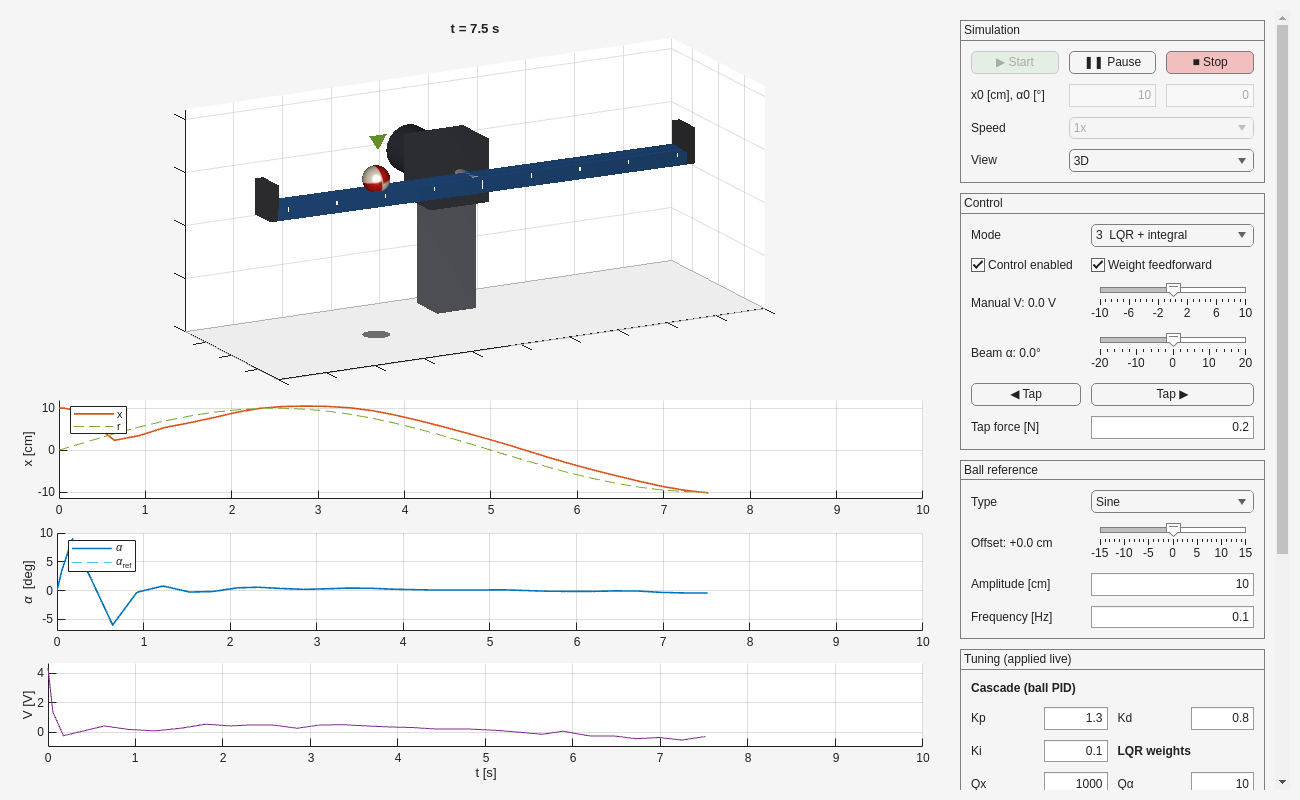
\includegraphics[width=\linewidth]{data/gui.png}
\caption{La GUI siguiendo en vivo una referencia senoidal de $\pm\SI{10}{cm}$ a \SI{0.1}{Hz} con el LQR.}
\label{fig:gui}
\end{figure}

\paragraph{La escena 3D.} La dibuja \code{bb\_draw}: la base, el pedestal, el motor con su reductora detrás de la viga, la viga (con una escala en centímetros y los topes de los extremos), la bola y su sombra. La bola tiene dos colores para que se vea rodar. El triángulo verde marca la referencia $r$. Se puede girar con el ratón o elegir otro punto de vista en la lista \textbf{View} (3D, \emph{Front}, \emph{Top}, \emph{Side}); desde código, con \code{bb\_view(ax, nombre)}.

\paragraph{Uso típico.}
\begin{enumerate}
  \item Elegir la posición inicial de la bola (cm) y el ángulo inicial de la viga ($^\circ$), y la velocidad de simulación.
  \item Pulsar \textbf{Start}. Desde ese momento, cualquier cambio de modo, referencia, tensión, ganancias de la cascada o pesos del LQR se aplica en vivo.
  \item Con la ventana activa, las teclas $\leftarrow/\rightarrow$ dan un golpecito a la bola hacia $-x$/$+x$ y, en el modo \code{beam}, $\uparrow/\downarrow$ cambian el ángulo de la viga en $\pm1^\circ$.
  \item La casilla \emph{Weight feedforward} activa o desactiva la compensación del peso de la bola (sección~\ref{sec:ff}).
  \item \textbf{Stop} y después \textbf{Export last run}: los datos quedan en \code{bb\_res} y se representan con \code{bb\_plot\_results}.
\end{enumerate}
